\chapter{Introduction}
\label{chap:introduction}

Robotic manipulation is a complicated problem in the field of robotics in which we want a robot to interact with and influence it's environment in a specific way to complete a task. This is much more complicated than simple robot locomotion, as we don't just want the robot to move and exist within in its environment, but instead we want the robot to have meaningful interactions with certain objects in the environment. These interactions may be complex involving many moving parts, or multiple individual objects entirely. Furthermore, these interactions may be unpredictable if the robot's actions are prone to failure, or if the robot is interacting with objects it has no prior knowledge of.\\

As currently described, this problem is not particularly hard to solve. One could spend a few hours hand crafting an exact set of instructions for the robot to complete, such that when run from start to finish the robot completes the task. However, this implementation is missing a crucial feature. It does not generalise to different environments. We want the robot to be able to complete the task even when the task is placed in a different environment. Specifically the robot should be able to analyse the state of the environment prior to or during the execution of the task and be able to adapt to this environment in order to complete the task.\\

Suppose we have a robot arm in which we can control the angle of each joint and an environment which contains a coffee mug. We could easily define the exact joint angles at each time step, such that when the robot executes these positions, it manages to pick up the mug. However, if we now change the environment, and move the mug to the side, then the robot is going to fail the task. It will follow the instructions as before, trying to pick up a mug that is no longer there. This control algorithm does not generalise to different environments, it is hard coded for one specific environment setup. We want a system which can sense the environment in some way, and change it's actions accordingly, making decisions based on the information from its sensors. For example seeing the mug has been moved to the side, and changing the joint angles such that it still manages to pick it up.\\

It is obvious that hard-coding the instructions for every possible task set up is intractable. The general approach to solving such a problem involves trying to teach the robot an understanding of the meaning behind the underlying task itself, abstracting it away from the environment it is performed in. For example, we do not want to teach the robot \speech{How do I pick up \textbf{\textit{this}} mug?} We want to teach it \speech{What does it mean to pick up \textbf{\textit{a}} mug?} and \speech{How do I know when I have picked up a mug?}. These success criteria questions are something we will refer back to when considering different algorithmic approaches in \refchap{chap:background}.\\

If the robot is able to comprehend this higher level notion of what it truly means to complete the task, without relying on environment specific information, then we have successfully extracted the task out from the environment. In this sense the task can be placed in any environment, and the concept of the task itself has not changed. The robot knows how to pick up a mug in whichever environment it is found in. The robot does not need to work out how to complete the task, it only needs to compute how to apply the already known task in this new unseen environment.\\

Some existing solutions to this problem \cite{rl, rl-intro-book, inverse-rl, behavioural-cloning, rl-book, behavioural-cloning-book} offload the work of extracting environment agnostic task information to the engineers. This requires us to formalise the task in a complicated mathematical expression which can be applied to any environment. This approach, called \socalled{Reinforcement Learning}, is detailed in \refsec{sec:reinforcement-learning}. Alternatively, engineers can directly generalise the task by presenting it in many different environments and demonstrating to the robot how to complete the task in each case. This however still multiplies the workload of engineers providing large amounts of training data to the system. This method, called \socalled{Imitation Learning}, is explored in \refsec{sec:imitation-learning}. \\

Newer state of the art solutions \cite{coarse-to-fine, one-shot-pose-estimate, one-shot-imitation} build on the ideas of Imitation Learning, but instead of offloading the work to the engineers, attempt to offload the work to an Artificially Intelligent system. A common approach among these solutions is to capture specialised additional information during training time which allows the task to easily generalise. This additional information, often in the form of images taken by the robot, is something which can be automatically collected with no extra effort from the engineers. In order to process and incorporate the additional information, these papers unanimously opt to rely on Artificial Intelligence models. Either training neural networks from scratch, or incorporating pre-trained vision transformer models. In doing so these solutions achieve a remarkable feat, in that a single human provided demonstration is sufficient to learn a task which generalises to unseen environments. We explore these \socalled{One-shot Imitation Learning} approaches further in \refsubsec{subsec:one-shot}. \reffig{fig:intro} illustrates the problem we aim to solve.\\

\begin{figure}[h]
    \centering
    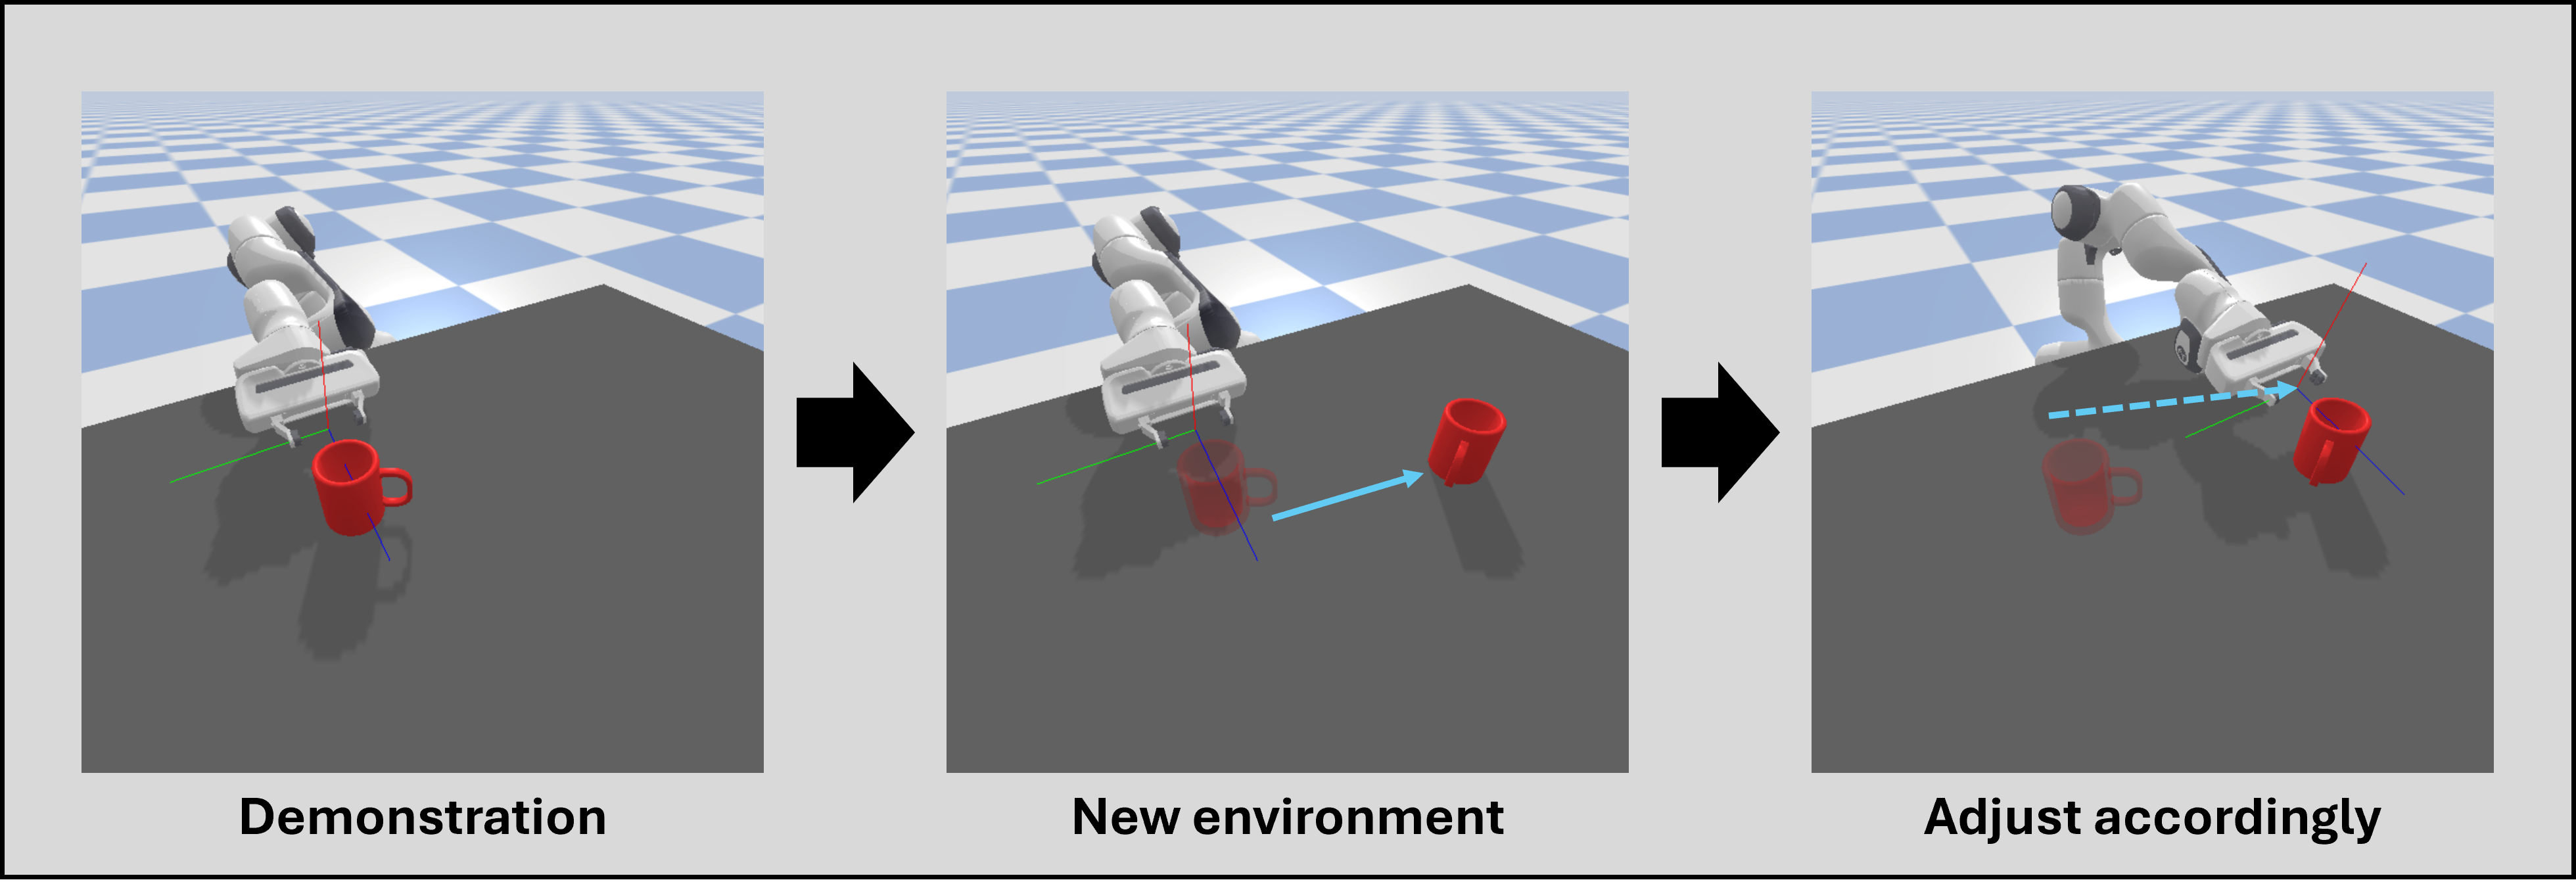
\includegraphics[width=\textwidth]{figures/intro.png}
    \caption{The One-shot Imitation Learning Problem}
    \label{fig:intro}
\end{figure}

\section{Contributions}
In this paper we consider the limitations of the aforementioned state of the art solutions. In particular we focus on \speech{DINOBot: Robot Manipulation via Retrieval and Alignment with Vision Foundation Models}, a system created by N. Di Palo and E. Johns \cite{one-shot-imitation} as a case study. N. Di Palo and E. Johns generously publicise their source code for installing and utilising the vision transformer at the heart of their system.\\

Upon implementing this system it becomes apparent that the physical hardware requirements of this and many other state of the art solutions are immense. The DINObot system requires in excess of 16GB of GPU video RAM. We are unable to find an exact requirement, since this has already reached the maximum hardware specifications of the machines available to us for this project. As such we were not able to implement the DINObot system at any point during this project. This unfortunately limits our ability to directly compare our solution to DINObot, since we cannot test DINObot on the same test suite we use to evaluate our own system. However it does highlight this issue, existing solutions are not accessible to a large portion of potential users.\\

The driving motivation for this paper is to emulate the methods of state of the art systems, to produce high quality and accurate results while operating under much tighter computational constraints. Our framework should be capable of learning tasks and generalising to novel environments from a single human provided demonstration. It should achieve this with substantially lower memory requirements, while not impacting performance and accuracy.\\

This paper manages to achieve a such a system, with comparable performance to existing solutions. One of the most significant features of the system presented in this paper is its ability to operate entirely on a CPU. The system performs efficiently without any GPU resources being utilised. Despite this the system is still fast enough for real time inference during testing. Our system combines strategies from existing One-shot Imitation Learning systems, while exchanging memory intensive Artificial Intelligence components for classical algorithms from the field of computer vision. While this may seem irrelevant in an application which already requires specialised robotics hardware, the methods described in this paper have broader applications in simulations, video games and pure mathematical settings. In such fields the reduced barrier to entry becomes highly desirable. Furthermore, as shown in this paper, physical robotics hardware has become a luxury as opposed to a necessity, with high quality simulation software providing a solid basis to perform robot learning within.\\

Moreover, we create a framework which can learn multiple tasks independently. The robot is able to identify which task to complete from its corpus of trained tasks, using only observations of the environment it finds itself in and no external input from a human. It can identify the task to complete by analysing the environment, and then executes this task in the specific test time environment. It achieves all of this with minimal pre-training, each learned task consisting of a single human provided demonstration combined with automatically collected data which facilitates the generalisation to novel environments. This data comes with no additional workload to the demonstrator.\\

\section{Ethical Considerations}
This project does not work directly with people or animals. However, there could be safety considerations if deploying to a physical robot arm. These potential safety concerns are a consequence of using any robot arm and are not specific to this project. As such normal safety protocol in remaining clear of the robot arm during operation would be sufficient.\\

There are no legal or licensing concerns with this project. All libraries used are open source and can be installed through the default Python package manager, pip.\\

A widely generalisable learning agent will be applicable to many scenarios and tasks, some of which may be malicious in nature. While it is possible that work from this project could be taken and misused to teach a robot morally questionable tasks, this is not the intended use or focus of this project.\\

Finally while this project does not directly focus on environmental issues, we should consider the energy used running the simulations and equipment. While this is a non-zero amount, it is for the purposes of research and well within reasonable limits. Furthermore, this paper specifically focuses on producing a robot learning algorithm with lower hardware requirements to run effectively. This allows our system to run on lower power and more efficient machines than previously possible. While this is undoubtedly a benefit of the solution presented, reducing the environmental impacts is not the focus of this paper.